%Physical principles

\section{Physical Principles}
\subsection{Standard Model}
\begin{figure}[hb]
	\centering
	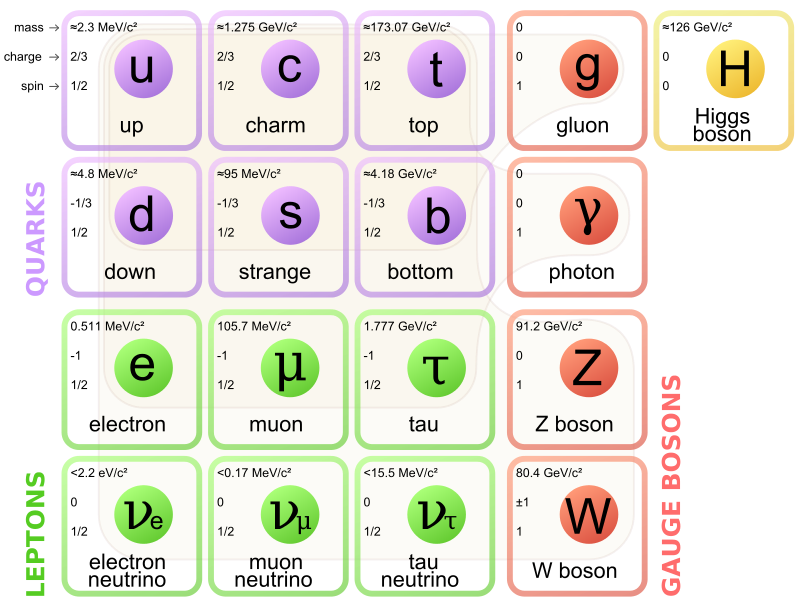
\includegraphics[scale=0.25]{graphics/Standard_Model_of_Elementary_Particles.png}
	\caption{Fundamental particles in the Standard Model}
	\label{fig:principles:Standard_Model_of_Elementary_Particles}
\end{figure}

Figure~\ref{fig:principles:Standard_Model_of_Elementary_Particles} gives an overview of the fundamental particles in the Standard Model. Quarks and Leptons obey the Pauli exclusion principle and are therefore fermions. Each of those also has a corresponding antiparticle with the same mass but opposite charge. Fundamental interactions are mediated by the Gauge Bosons, namely two particles interact with each other by exchanging said bosons. The original theory stated that fermions and bosons are massless, they gain mass via the Higgs-Kibble mechanism which implies the existence of another particle, the Higgs Boson\cite{muenchen}.

\subsection{Electroweak force and Weinberg Angle}
1967 Glasgow, Salam and Weinberg were able to unify the electromagnetic and weak force. In this model the electroweak interaction is mediated by four Bosons $W^1$, $W^2$, $W^3$ and $B^0$. The Bosons of the Standard Model are then described as a linear combination of those Bosons\cite{Grif}:
\begin{equation}
\begin{aligned}
\gamma &= B^0 cos(\theta_w) + W^0 sin(\theta_w) \\
Z^0 &= -B^0 sin(\theta_w) + W^0 cos(\theta_w)
\end{aligned}
\end{equation}
\begin{equation}
sin^2(\theta_w)+cos^2(\theta_w) = \frac{\pi\alpha}{\sqrt{2}G_FM_Z^2}
\end{equation}
\begin{equation}
M_W = M_Z~cos(\theta_w)
\end{equation}

\subsection{$e^-e^+$ Interactions}
\paragraph{$e^-e^+ \rightarrow e^-e^+$}

%stelle finden
\begin{figure}[hb]
	\centering
	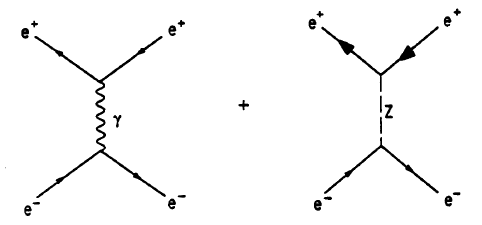
\includegraphics{graphics/BhabbaStreuung.png}
	\caption{Feynman diagrams of the $e^-e^+ \rightarrow e^-e^+$ scattering (t-channel)}
	\label{fig:principles:BhabbaStreuung.png}
\end{figure}
 
\paragraph{$e^-e^+ \rightarrow f^-f^+$}
\begin{figure}[hb]
	\centering
	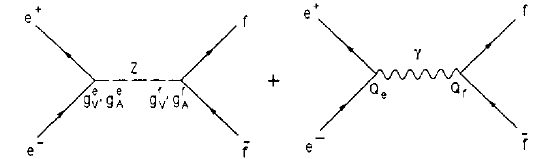
\includegraphics{graphics/annihilation.png}
	\caption{Feynamn diagram of the $e^-e^+ \rightarrow f^-f^+$ in first order, where f is an arbitrary fermion}
\end{figure}

\subsection{Cross Section}
\begin{equation}
\sigma = \frac{N}{\int L~\text{d}t}
\end{equation}

\subsection{Forwards-backwards Asymmetry}
\begin{equation}
\sigma_f=\int_{0}^{1}\frac{\text{d}\sigma}{\text{d}cos(\theta)}~\text{d}cos(\theta) \\
\sigma_b=\int_{-1}^{0}\frac{\text{d}\sigma}{\text{d}cos(\theta)}~\text{d}cos(\theta)
\end{equation}
\begin{equation}
A_{fb}=\frac{\sigma_f-\sigma_b}{\sigma_f+\sigma_b}
\end{equation}
